\documentclass[letterpaper,10pt]{article}
\usepackage[small,bf]{caption}
\usepackage{amssymb,amstext,amsmath,amsthm,hyperref,sidecap,wrapfig,listings}
\usepackage{setspace,alltt,algorithm,verbatim,theorem,appendix,textcomp}
\usepackage{algpseudocode,graphicx,subfig,fullpage,fancyhdr,lastpage}
\usepackage{setspace}

% Setup document
\DeclareGraphicsExtensions{.png}
\numberwithin{equation}{section}
\setlength{\headheight}{12pt}
\setlength{\headsep}{15pt}
\pagestyle{fancy}
\lhead{CCMP Agent}
\chead{\Large{\textbf{SYSC 5103: Project Report}}}
\rhead{\today}
\lfoot{}
\cfoot{\thepage~of~\pageref{LastPage}}
\rfoot{}
\begin{document}

\section{Introduction}
The CCMP Agent, for the ART testbed, is a framework that uses two components to
control its behaviour in an evolving multi-agent environment: the Trust Network
and the Decision Tree.  The trust network manages and updates the trust values
for each agent in the ART testbed. The decision tree provides a methodolgy for
the agent to make decisions on the actions to take based on the knowledge in the
trust network. 

In this project an abstract agent framework was developed to provide the
interactions with the ART testbed and other agents.  This framework makes use
of Java interface classes to work with abstract implementations of the trust
network and decision tree components.  To implement an accurate trust network a
baysian approach was used based on the paper B-trust: Bayesian Trust Framework for Pervasive
Computing.  To provide a flexible decision tree environment the Weka Java API
was used to design and execute decision tree graphs.

\section{CCMP Agent Framework}
The ART testbed provides a base Agent class with several functions that must be
implemented by the new agent. These functions allow the agent to interact with
the other agents and participate in the game through the exchange of differet
messages.  

To facilitate the distributed development environment it was important to break
the agent environment into different parts.  The CCMP Agent consists of the
base CCMP Agent class, base Trust Network interface class, an base Decision
Tree interface class and their associated implementations.

\subsection{Main Agent}
The base framework class, CCMPAgent, is the subclass of the ART testbed Agent
and provides the interface to the ART testbed.  The CCMPAgent is
responsible for handling the generation, parsing and responses to the
messages within the testbed Agent methods.  

It does this in a similar and abstact manner for each one. First it parses the
incoming messages and updates the trust network and decision tree on the
results of the messages, either positive or negative.  After updating the
knowledge base regarding the actions of the other agents and passing the new
values from the trust network to the decision tree if queries the decision tree
to determine what action to take.  It then generates the appropriate
messages and passes them to the sim.

The base CCMPAgent class implements all this functionality in an abstract way
using the base TrustNetwork and DecisionTree classes.  The specific objects
types, such as the Bayesian trust network and Weka decision tree, are
instantiated in subclasses of CCMPAgent.  It is these subclasses that are passed
to the ART testbed for creation in the sim.  In this manner different
implementations of the trust network and decision tree classes can be easily
incorperated into the CCMPAgent.

\begin{center}
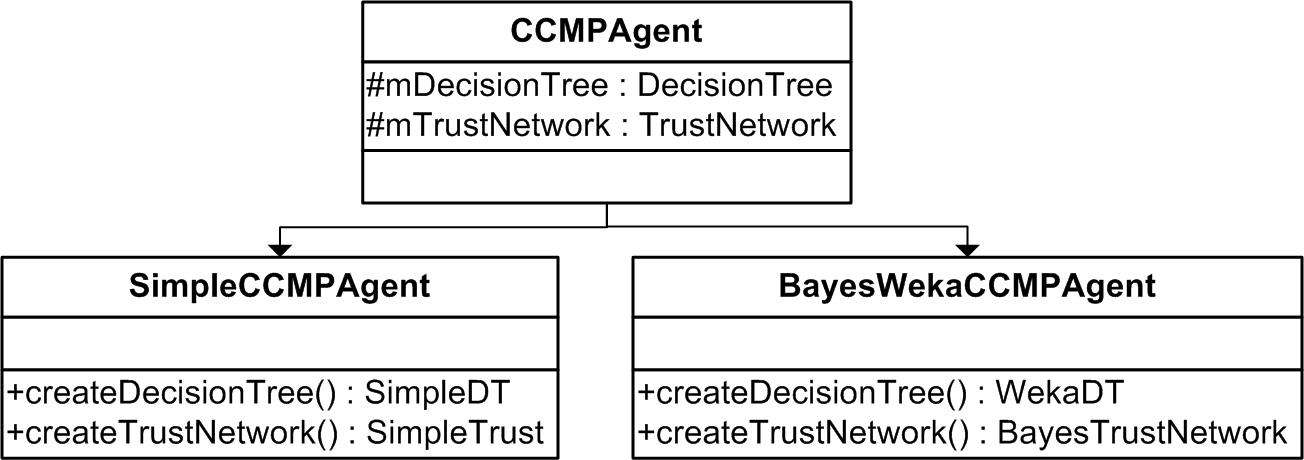
\includegraphics{images/CCMPClasses.jpg}
\end{center}

\subsection{Trust Network}
The trust network is an abstract class used to represent the trust the agent
has for other players.  The interface class provides methods to update the
trust values based on events in the sim, such as receiving new reputation
information from other agents or negative actions by an agent.  At the end of
each frame the resulting final appraisal and each agents opinion are also
passed to the trust network as they could be used to update trust values.

The trust network also allows for the representation of inferred trust, or the
trust we believe an other agent has for us.  This value could be used by the
decision tree to affect decisions and can be modelled both by asking the other
agent about our reputation and by keeping track of our actions to the specific
agent.  To this end several methods are provided that will tell the trust
network about the actions the CCMPAgent has taken, such as not providing the
requested information or modifying the appraisal value.

\begin{center}
\begin{array}{cc}
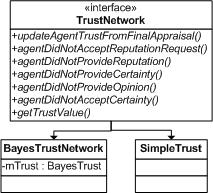
\includegraphics{images/TrustNetworkClasses.jpg} &
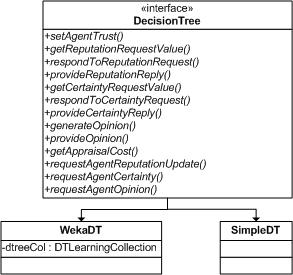
\includegraphics{images/DTClasses.jpg}
\end{array}
\end{center}

\subsection{Decision Tree}
Abstract class that provides direction to the agent on how to behave.  For each
possible action (list actions) the DT has a function to provide direction to
the main agent class.


\section{Baysian Trust Network}
Here you talk about the Baysian Trust Network \cite{btrust}.

\begin{figure}[h]
\begin{equation}
mean = \sum_{j=0}^{n-1}{(j)(d_j)}
\end{equation}
\end{figure}

\begin{figure}[h]
\begin{equation}
variance = \bigg(\sum_{j=0}^{n-1}{(j^2)(d_j)} \bigg) - mean^2
\end{equation}
\end{figure}



\section{Weka Decision Tree}
The decision was made early that developing an advanced tree classifier from scratch would
be unnecessary as the Weka 3.6.1\cite{weka} open source library already provided an implementation that meet
all the requirements.  These requirements including being able to classify data sets and 
then being able to query the resulting tree to determine the categorical action based on the set
of non-categorical test.  Also, there was a need to view the resulting tree for visual inspection.

\subsection{Interfacing with Weka}
In order to increase the reusability of the decision tree library, classes were created that 
reproduce the components of the Weka Attribute-Relation File Format (ARFF) instead of merely
storing the contents of an ARFF file.  These classes are of this decision tree library, dtlib, 
are described in the following Table~\ref{table:attribs}.

\begin{table}[h]
\label{table:attribs}
\centering
\begin{tabular}{|l|p{5in}|}
\hline
DTAttribute &
Contains two strings representing the name of the attribute and its type.
The type can be either 'numeric' or some enumerated set of the form '\{enum1,enum2,etc\}'.\\
\hline
DTWekaARFF &
Contains a string for the name of the tree, a vector of the non-categorical attributes and the 
categorical attribute as the last element, and a String array representing the data that the 
decision tree will be built from.\\
\hline
DTLearning &
Contains a DTWekaARFF object and a J48 tree object.  The tree object is retrieved by converting
the DTWekaARFF element to the ARFF format and passing it to Weka's 'buildClassifier' function.  
Test are simply a comma separated string of non-categorical data and a '?' for the categorical 
attribute.  The 'DTClassify' method takes this string and creates a proper ARFF format query.
This is then passed to Weka's 'classifyInstance' which returns a double values.  This double value
represents the enumerated string specified in the type of the categorical attribute.  This value is
used to parse the type string and then the appropriate string is returned.  \\
\hline
DTLearningCollection &
Extends Vector to only contain DTLearning objects.\\
\hline
\end{tabular}
\caption{Decicion Tree library classes}
\end{table}

\subsection{XML declaration}

The decision trees were stored in the configuration XML allowing the behaviour of an agent to be change without
recompiling the entire project.  This flexibility was achieved by structuring the classes so that 
they could be built using the Digester XML parser.  This meant that any decision tree could be modified in 
terms of their non-categorical but the categorical attribute must agree with what is currently within the 
compiled code.  If a new non-categorical attribute was required for a decision tree, then the compiled code would
have to be adapted to know how to retrieve the values of that attribute.

\subsection{Integration with Agent}

The agent contains a class, WekaDT, that contains the constructed decision trees.  This class only has
the necessary methods to retrieve the data necessary to build a test used to query any of the decision
trees.  There is a single private method, 'BuildTest' that will construct test for each tree, this allows the flexibility
of adding non-categorical attributes without adjusting the compiled code.  This method is capable of
examining the current decision tree to determine which non-categorical attributes it contains.

Whenever the agent determines which action to take, it calls the appropriate method for the decision 
tree.  This method calls 'BuildTest' to construct the appropriate which is then queried to the
appropriate tree.  There is then a if-else sequence that based on the returned classified string
will return the proper value.

\subsection{Example}

\begin{figure}[h]
  \centering
  \label{fig:xml2dt}
  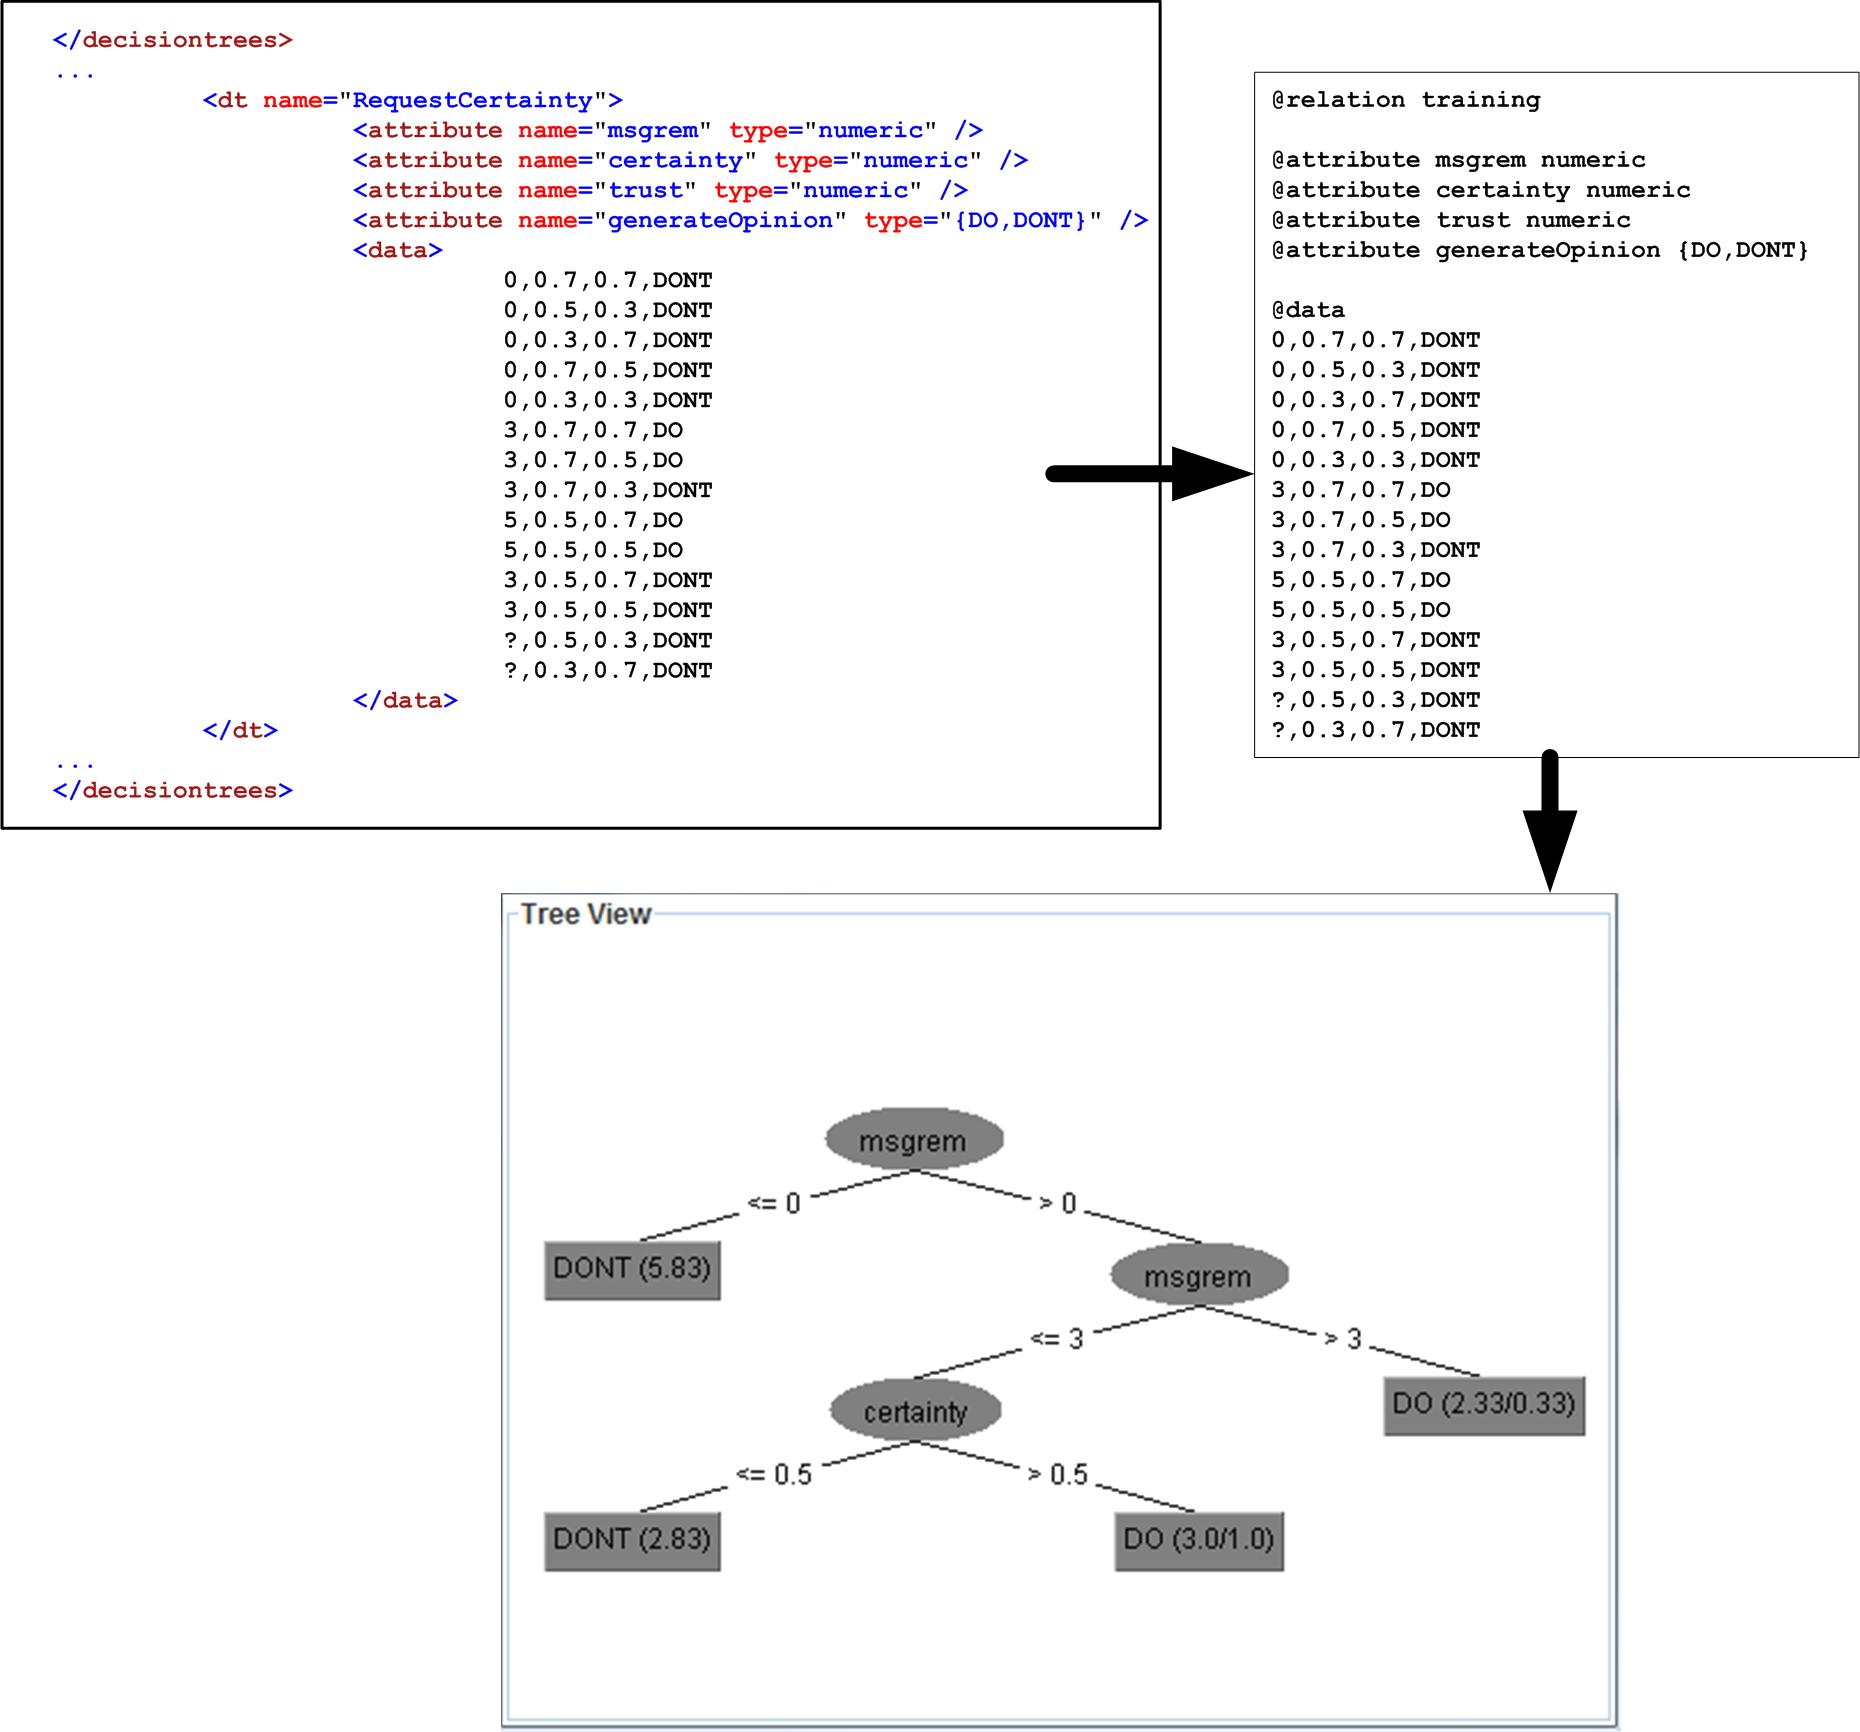
\includegraphics[width=1\textwidth]{../projectPres/images/xml2dtxtra.jpg}
  \caption{XML gets converted to the Weka ARFF format and can then be visualized.}
\end{figure}

\begin{figure}[h]
  \centering
  \label{fig:xml2dttest}
  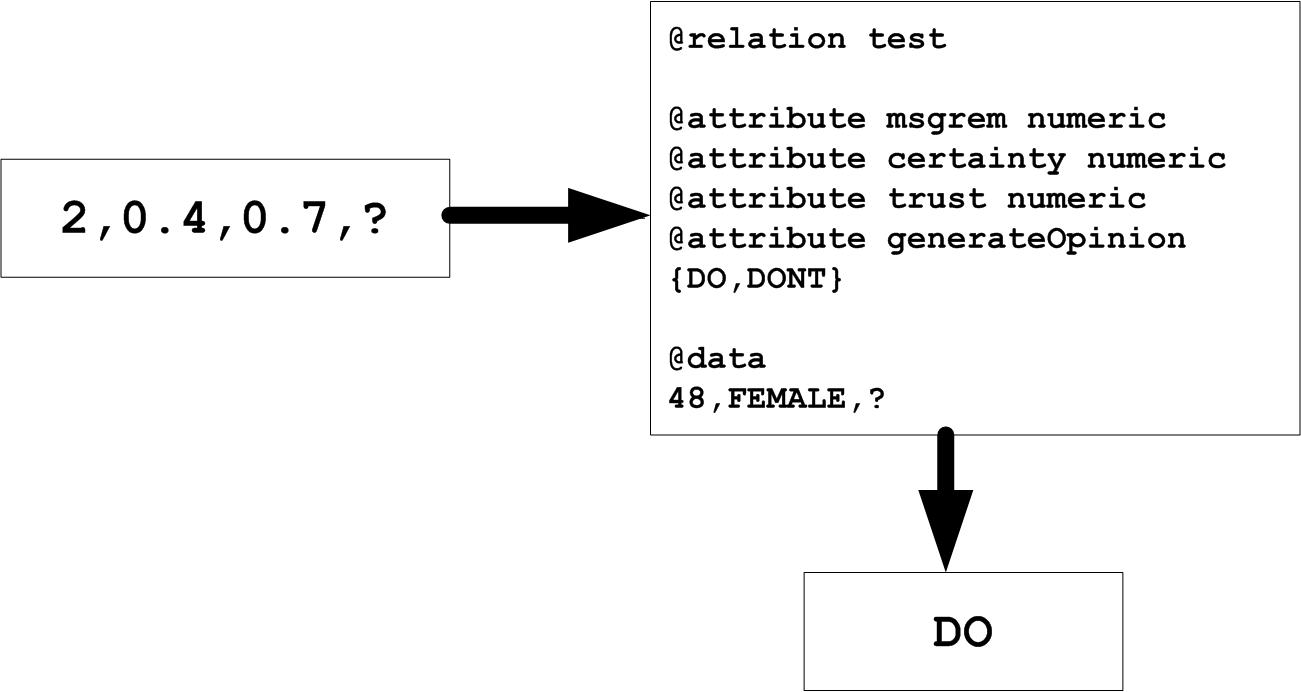
\includegraphics[width=1\textwidth]{../projectPres/images/xml2dttest.jpg}
  \caption{Comma separated test gets converted to the Weka ARFF format and then gets classified for 
  the tree shown in \ref{fig:xml2dt}.}
\end{figure}

\ref{fig:xml2dt} shows a sample decision tree how the shown decision tree can be described in XML.  
In \ref{fig:xml2dttest} there is a sample comma separated test and its classified return value.

\subsection{Testing and Development of Decision Trees}
Testing was accomplished by first developing a method that opened a Java window and used the Weka
'TreeVisualizer' class to visualize the developed tree.  An application was then written that listed
all the decision trees that were required by the Agent.  Attributes and Data were selected and then 
once the application was run the Weka constructed trees could be visually inspected to ensure that
they met the desired behaviour.

Some workarounds were necessary to properly interface with the Weka library.  Weka functions are
designed to expect Strings of the input file and not simply text reprenting the ARFF format, thus
the DTWekaARFF converted string was then converted to a StringReader which Weka could accept.

The tree classification algorithm used was J48 mainly due its ability to be visualized once constructed.
However, some of the generated trees did not classify data properly resulting in trees that did not
meet the desired behaviour.  By repeating training data entries twice, the J48 algorithm produced
trees that met expected results. 

\section{Test Methodologies}
To test the behaviour and stability of the CCMP Agent framework and the
associated decision tree and trust network implementations several different test
strategies were adopted.

\subsection{CCMP Agent Framework Testing}
The CCMP Agent Framework was first tested by implementing the
Simple Agent example provided in the ART testbed.  A SimpleDT and
SimpleTrust implementation of the associated interface classes were created.
The SimpleDT class implemented the decision methods using the same if conditions
as the example agent.  The SimpleTrust class merely provided trust values of
1.0, the same as the example agent.  A SimpleCCMPAgent was then created that
instantiates the SimpleDT and SimpleTrust classes.  The behaviour of the
SimpleCCMPAgent was then compared to the behaviour of the example SimpleAgent
to ensure the CCMP Agent Framework implemented the ART methods correctly.

Logging to a file was also implemented in the CCMPAgent class.  The CCMPAgent
class will print information on the messages received, decisions taken and the
messages generated.  It also logs any negative actions taken by other agents.
With the use of logging, the complete behaviour of the SimpleCCMPAgent and
associated  could be examined to ensure the expected behaviour was being
performed.

\subsection{Weka Decision Tree Testing}
The Weka Decision Tree implementation was tested in two ways.  The first
method was to create classes that would test the parsing of the XML config
file, which contains the Weka data, and to test the creation and execution of
the Weka decision tree parsing.

The second requirement for testing of the Weka Decision Tree was to ensure
that the behaviour of the Weka decision trees generated from the Weka data
provided in the XML config file was as expected.  To speed up the process of
verifying the Weka decision trees a class was created to visualize the Weka
decision trees.  The XML config file is parsed, Weka decision tree created and
then displayed using the Weka visualization tools.

\subsection{Bayes Trust Framework Testing}
The Bayesian trust component of the project was quality-checked by unit testing.
Using the JUnit testing framework, we built unit tests for all 13 of our concrete
classes in the Bayesian trust library. These tests include positive tests, which
check for correct behaviour, and negative tests, which ensure correct error
handling under exceptional conditions. The tests were also useful as regression
tests, i.e., to ensure that previously fixed bugs are not reintroduced as a
result of new code. In total, we have 58 test cases which verify the Bayesian
trust library.



\newpage
\bibliographystyle{ieeetr}
\bibliography{references}

\end{document}